\documentclass[12pt, letterpaper]{article}
\usepackage[titletoc,title]{appendix}
\usepackage{color}
\usepackage{booktabs}
\usepackage[tableposition=top]{caption}
\newcommand\fnote[1]{\captionsetup{font=small}\caption*{#1}}

\usepackage[usenames,dvipsnames,svgnames,table]{xcolor}
\definecolor{dark-red}{rgb}{0.75,0.10,0.10} 
\usepackage[margin=1in]{geometry}
\usepackage[linkcolor=dark-red,
            colorlinks=true,
            urlcolor=blue,
            pdfstartview={XYZ null null 1.00},
            pdfpagemode=UseNone,
            citecolor={dark-red},
            pdftitle={Partisan Vision}]{hyperref}
%\usepackage{multibib}
\usepackage{geometry} % see geometry.pdf on how to lay out the page. There's lots.
\geometry{letterpaper}               % This is 8.5x11 paper. Options are a4paper or a5paper or other... 
\usepackage{graphicx}                % Handles inclusion of major graphics formats and allows use of 
\usepackage{amsfonts,amssymb,amsbsy}
\usepackage{amsxtra}
\usepackage{natbib}
\DeclareRobustCommand{\firstsecond}[2]{#1}
\usepackage{verbatim}
\setcitestyle{round,semicolon,aysep={},yysep={;}}
\usepackage{setspace}             % Permits line spacing control. Options are \doublespacing, \onehalfspace
\usepackage{sectsty}             % Permits control of section header styles
\usepackage{lscape}
\usepackage{fancyhdr}             % Permits header customization. See header section below.
\usepackage{url}                 % Correctly formats URLs with the \url{} tag
\usepackage{fullpage}             %1-inch margins
\usepackage{multirow}
\usepackage{rotating}
\setlength{\parindent}{3em}
\usepackage{subcaption}

%\usepackage[T1]{fontenc}
%\usepackage{bm}
\usepackage{lmodern}
%\usepackage{libertine}
%\usepackage{gfsdidot}
\usepackage{chngcntr}

\title{Partisan Vision? Partisan Bias in Simple Visual Evaluations}

\author{Carrie Roush\thanks{Carrie can be reached at, \href{mailto:carolyn.roush@gmail.com}{\texttt{carolyn.roush@gmail.com}}} \and 
Gaurav Sood\thanks{Gaurav can be reached at, \href{mailto:gsood07@gmail.com}{\texttt{gsood07@gmail.com}}} \and 
Alex Theodoridis\thanks{Alex can be reached at \href{alexandertheodoridis@gmail.com}{\texttt{alexandertheodoridis@gmail.com}}}}

\begin{comment}

setwd(paste0(githubdir, "partisan_vision/ms/"))
tools::texi2dvi("partisan_vision.tex", pdf = TRUE, clean = TRUE)
setwd(githubdir)

\end{comment}

\begin{document}
\maketitle
\thispagestyle{empty}

\begin{abstract}

\noindent In the current era of partisan polarization, partisanship strongly colors partisans' worldviews. But does it cause partisans to \textit{see} different things? We test the hypothesis using two different experiments and a survey. The data suggest that the effect is generally small.
\end{abstract}

\newpage

\doublespacing

Partisans are increasingly polarized \cite{IyengarSoodLelkes2012} with partisan cleavages outstripping some of the longer-standing racial cleavages. In this paper, we explore whether polarization affects how partisans `see.' We test the hypothesis with simple visual evaluative tasks. In particular, we field two survey experiments and a survey. We find that partisan bias is generally small.

\section{Data and Research Design}
To assess how partisans \textit{see}, we fielded two survey experiments on a nationally representative sample of people selected by YouGov \citep{rivers2007} as part of a Cooperative Congressional Election Study (CCES) module. In the first experiment, we presented people with a short passage and asked them to count the number of errors in it. We manipulated the perceived party of the person writing the text (see Figure~\ref{fig:mistakes_dem}). In the second experiment, we showed people a photo of a parking lot and asked them to estimate the number of poorly parked cars. We manipulated which parties' members parked the car by manipulating the caption indicating where the photo was taken (see Figure ~\ref{fig:parking_treat_dem}). We replicated the first experiment on Lucid.

We complemented the survey experiments with a partisan evaluative task on a survey. In a survey conducted on MTurk, we asked respondents to watch a short video and estimate how many people in the video were wearing masks. In particular, our directions were as follows: ``Please watch the following short (10-second) video. You will be asked a question about it on the next screen. ...How many people in the video were wearing masks?''

\section{Results}

As Table~\ref{tab:error_sum_cces} shows, Democrats find 9.7 mistakes when they think the text is written by a Democrat compared to 9.9 mistakes when they think the text is written by a Republican (see also Figure ~\ref{fig:text_cces}). On the other hand, Republicans find 8.4 mistakes on average when they think the text is written by a Democrat and 8.1 mistakes when they think it is written by a Republican. And while the differences are consistent with partisan bias, the differences are small. The point is especially clear when you look at the medians, which are the same.

% latex table generated in R 4.3.0 by xtable 1.8-4 package
% Mon Jun 26 17:56:16 2023
\begin{table}[!htb]
\centering
\caption{Average Number of Writing Errors} 
\label{tab:error_sum_cces}
\begin{tabular}{llrrrr}
  \hline
pid3lean & Error\_split & avg & med & n & std\_error \\ 
  \hline
Democrat     & DEM & 9.7 & 10.0 & 334 & 0.2 \\ 
  Democrat     & REP & 9.9 & 10.0 & 324 & 0.2 \\ 
  Independent  & DEM & 9.7 & 10.0 & 94 & 0.5 \\ 
  Independent  & REP & 9.2 & 9.0 & 110 & 0.4 \\ 
  Republican   & DEM & 8.4 & 8.0 & 253 & 0.3 \\ 
  Republican   & REP & 8.1 & 8.0 & 252 & 0.3 \\ 
   \hline
\end{tabular}
\end{table}


Table ~\ref{tab:error_sum_lucid} presents the results of the replication on Lucid. Democrats find 5.5 (.6) errors on average when they think Democrats wrote the text vs. 5.9 (.8) when they think Republicans wrote it. On the Republican side, the corresponding numbers are 5.6 (.9) (when they think Democrats wrote the text) vs. 4.9 (.3) (when they think Republicans wrote it) (see also Figure ~\ref{fig:text_lucid}).

% latex table generated in R 4.3.0 by xtable 1.8-4 package
% Mon Jun 26 18:11:58 2023
\begin{table}[!htb]
\centering
\caption{Average Number of Writing Errors (Lucid)} 
\label{tab:error_sum_lucid}
\begin{tabular}{llrrrr}
  \hline
pid3 & edit\_cond & mean\_mis & med\_mis & n & std\_error \\ 
  \hline
dem & d & 5.5 & 5.0 & 177 & 0.6 \\ 
  dem & r & 5.9 & 5.0 & 132 & 0.8 \\ 
  ind & d & 4.6 & 4.0 & 73 & 0.3 \\ 
  ind & r & 5.3 & 5.0 & 72 & 0.3 \\ 
  rep & d & 5.6 & 4.0 & 111 & 0.9 \\ 
  rep & r & 4.9 & 5.0 & 109 & 0.3 \\ 
   \hline
\end{tabular}
\end{table}


We see a slightly larger partisan bias in the experiment that manipulates which party's members parked the cars. Democrats on average believe there are 6.1 poorly parked cars outside the Democratic Party meeting while they think there are 8.7 poorly parked cars in front of the Republican Party meeting (see Table ~\ref{tab:parking_sum_cces}) (see also Figure ~\ref{fig:parking_cces}). As above, the medians are much closer at 5 and 6 for the Democratic Party meeting and the Republican Party meeting respectively. Switching to Republicans, the gap is much narrower---Republicans on average think that there are 8.7 poorly parked cars in front of the Democratic Party meeting and 8.1 in front of the Republican Party meeting. The gap in medians is 1. The results from Independents make interpretation slightly complicated as Independents show a pronounced pro-Republican bias. One plausible explanation is `hidden Republicans' among Independents.

% latex table generated in R 4.3.0 by xtable 1.8-4 package
% Mon Jun 26 17:56:16 2023
\begin{table}[!htb]
\centering
\caption{Average Number of Parking Errors} 
\label{tab:parking_sum_cces}
\begin{tabular}{llrrrr}
  \hline
pid3lean & UCMParking\_split & avg & med & n & std\_error \\ 
  \hline
Democrat     & Democratic Party & 6.1 & 5.0 & 211 & 0.4 \\ 
  Democrat     & Republican Party & 8.7 & 6.0 & 212 & 0.6 \\ 
  Independent  & Democratic Party & 10.9 & 7.0 & 57 & 1.5 \\ 
  Independent  & Republican Party & 6.7 & 5.0 & 61 & 0.9 \\ 
  Republican   & Democratic Party & 8.4 & 6.0 & 181 & 0.6 \\ 
  Republican   & Republican Party & 8.1 & 5.0 & 163 & 0.7 \\ 
   \hline
\end{tabular}
\end{table}


Turning to the results from the MTurk survey, we see that results are again muted (see Table ~\ref{tab:trump_sum}). (We winsorized the responses because of absurd responses like 80,000.) We would have expected large differences between Democrats and Republicans but instead, we see that the means are roughly the same.

% latex table generated in R 4.2.2 by xtable 1.8-4 package
% Sun Nov 27 23:33:13 2022
\begin{table}[!htb]
\centering
\caption{Number of People Wearing Masks} 
\label{tab:trump_sum}
\begin{tabular}{lrrrrr}
  \hline
pid\_dem\_l & p\_25 & p\_50 & p\_75 & n & std\_error \\ 
  \hline
democrat & 1.0 & 1.0 & 5.0 & 919 & 3.0 \\ 
  independent & 1.0 & 1.0 & 5.0 & 111 & 3.0 \\ 
  republican & 2.0 & 2.0 & 6.0 & 879 & 4.0 \\ 
   \hline
\end{tabular}
\end{table}


\clearpage
\bibliographystyle{apsr}
\bibliography{vision}
\clearpage


\appendix
\renewcommand{\thesection}{SI \arabic{section}}
\setcounter{table}{0}\renewcommand\thetable{\thesection.\arabic{table}}  
\setcounter{figure}{0}\renewcommand\thefigure{\thesection.\arabic{figure}}
\counterwithin{figure}{section}

\section{Treatments}
\begin{figure}[!htbp]
\centering
\caption{Text Treatment}
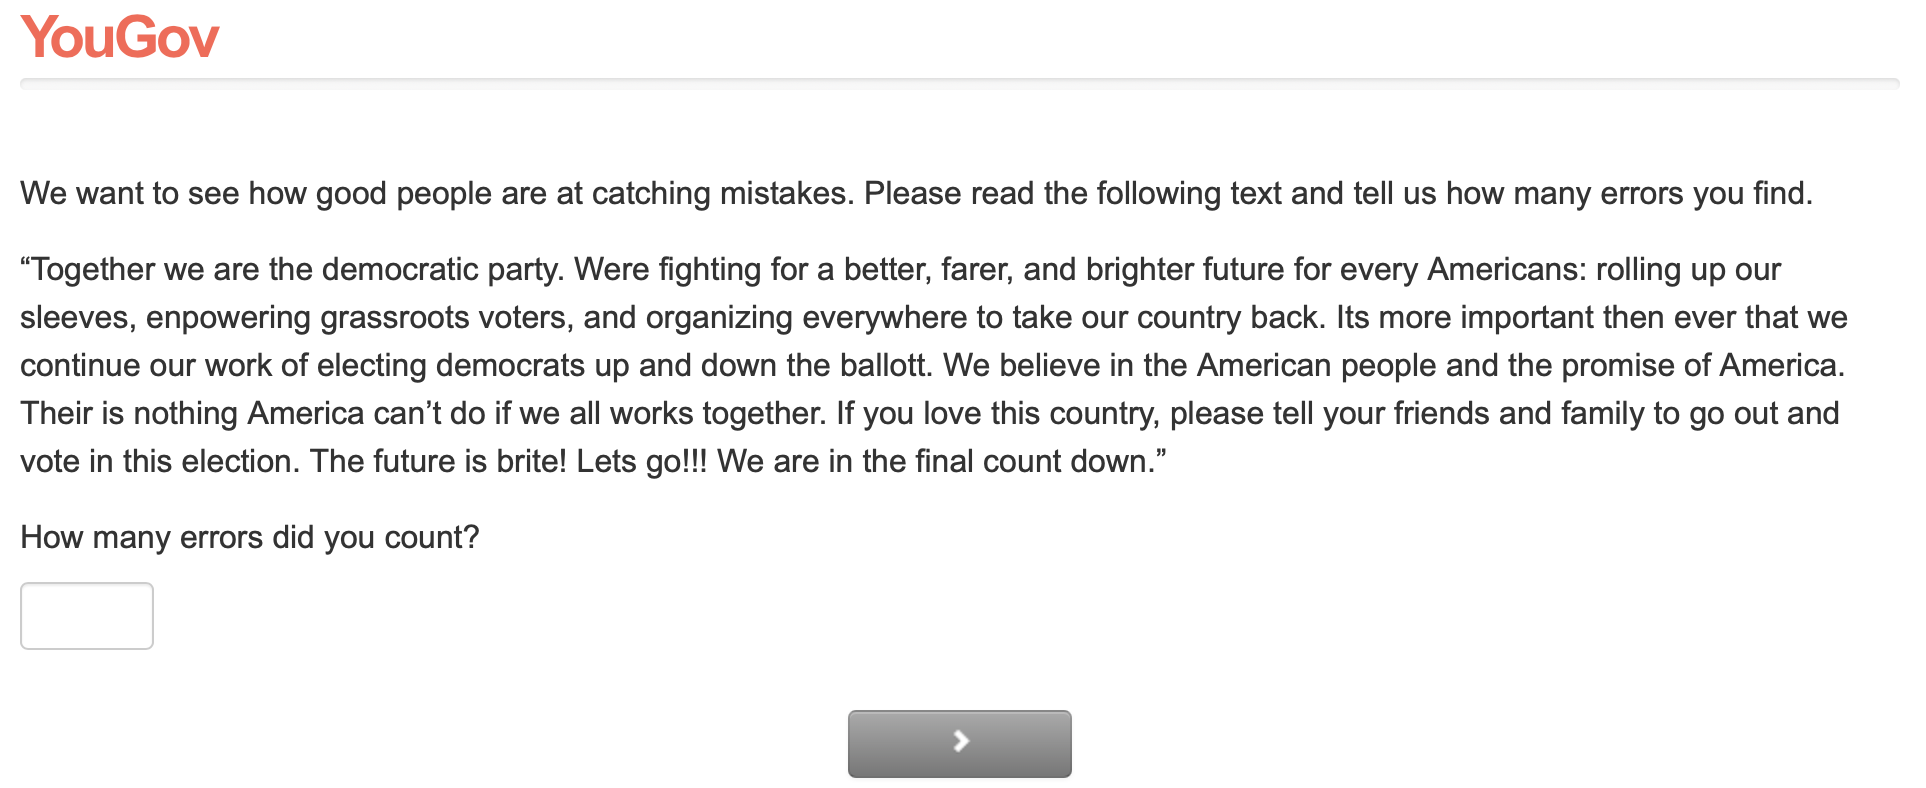
\includegraphics[scale=.4]{../data/treats/Mistakes_Dem.png}
\label{fig:mistakes_dem}
\end{figure}
\begin{figure}[!htbp]
\centering
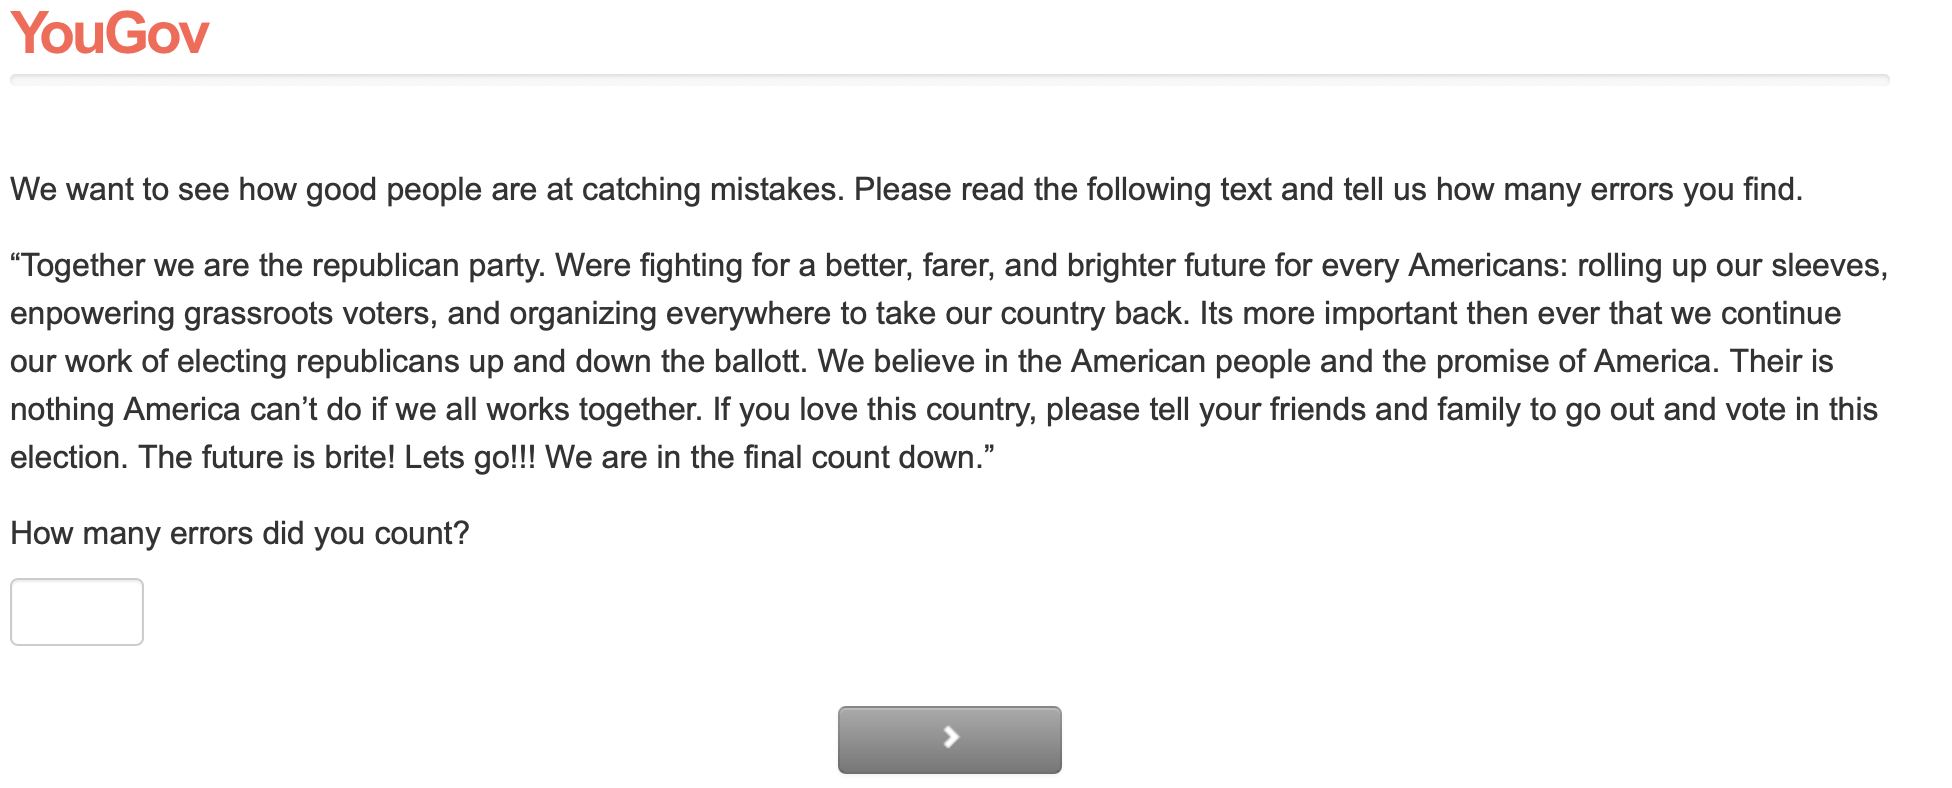
\includegraphics[scale=.4]{../data/treats/Mistakes_Rep.png}
\label{fig:mistakes_rep}
\end{figure}

\clearpage
\begin{figure}[!htbp]
\centering
\caption{Parking Lot}
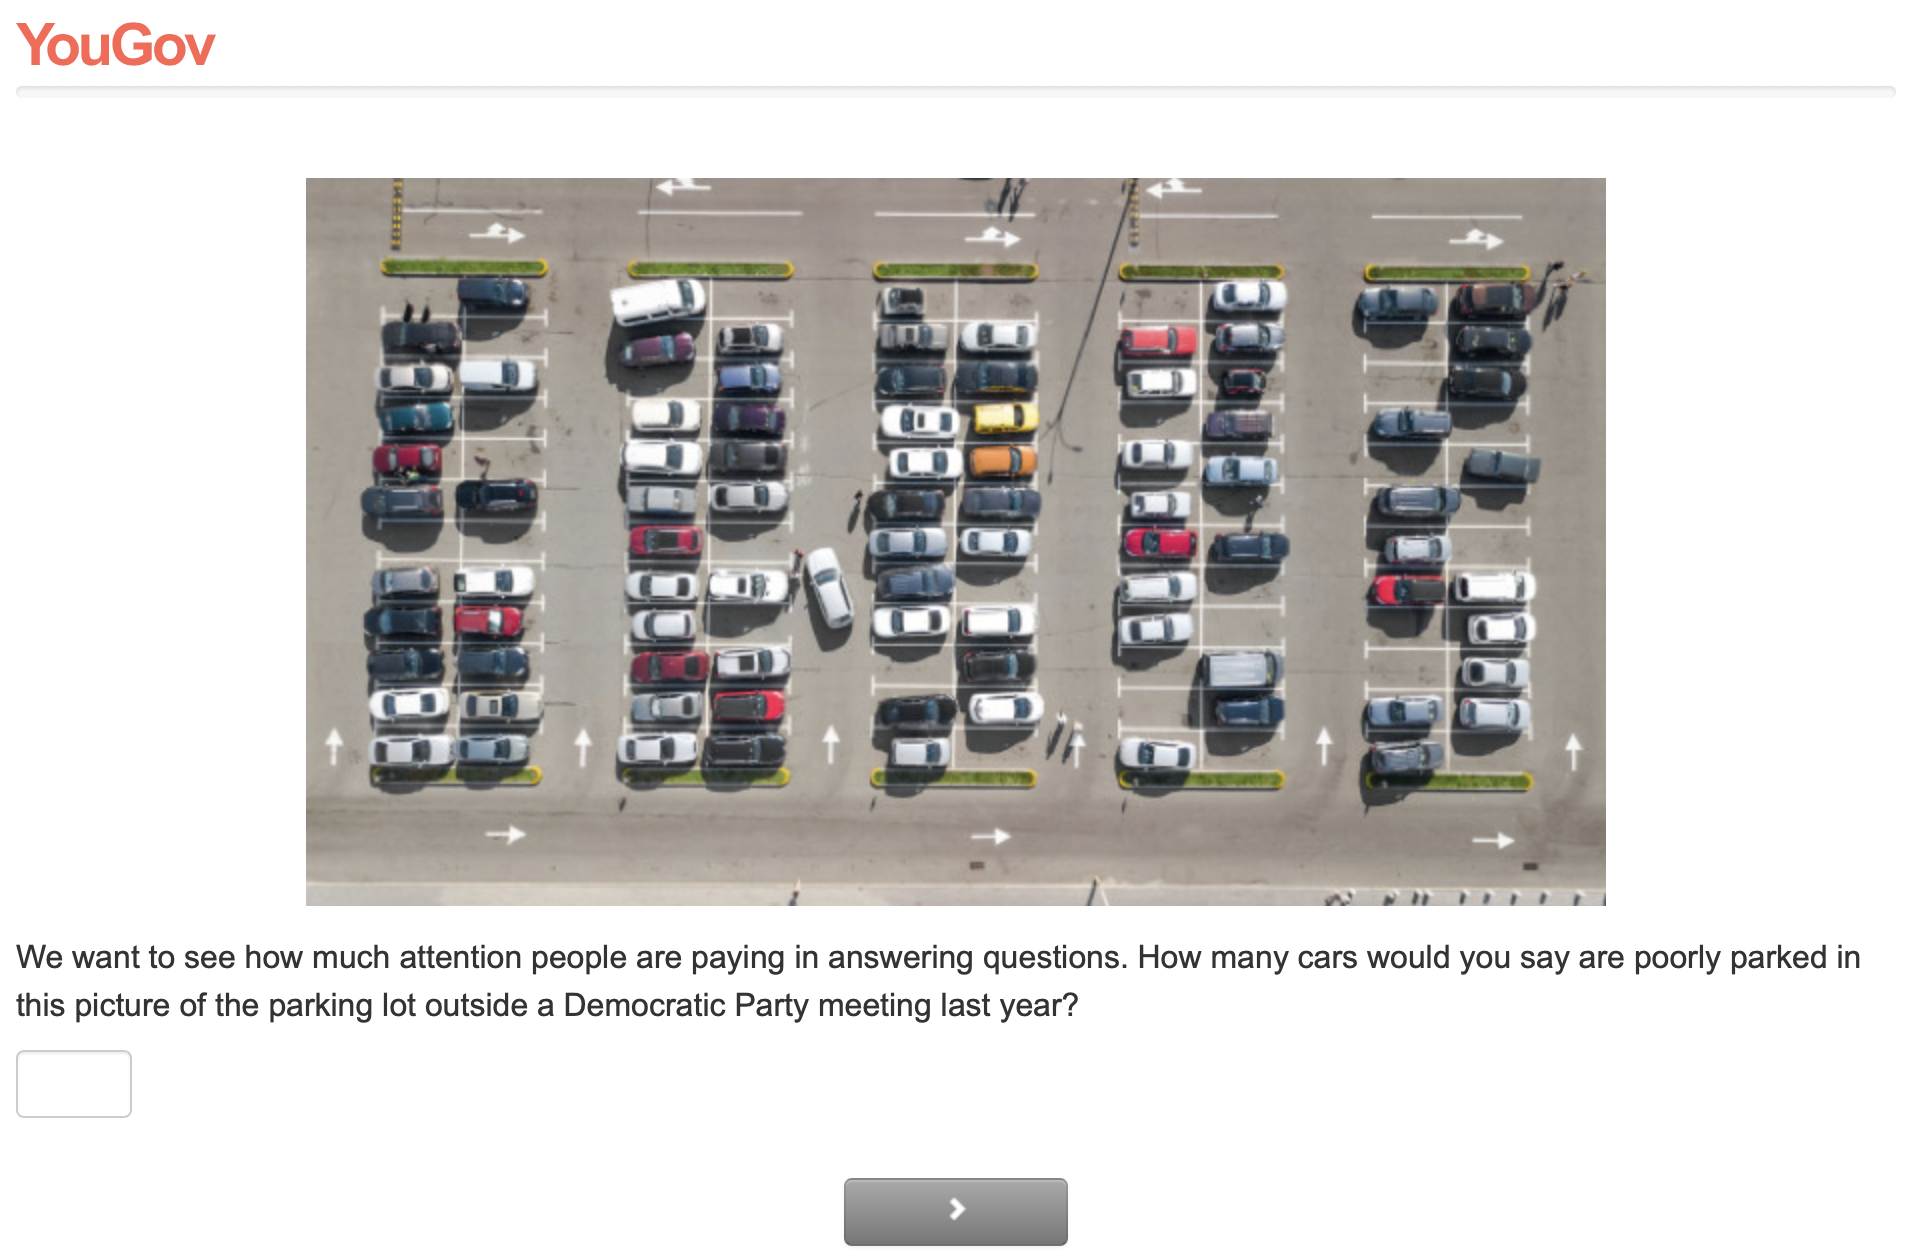
\includegraphics[scale=.4]{../data/treats/Parking_Lot_Dems.png}
\label{fig:parking_treat_dem}
\end{figure}

\clearpage

\section{Figures}

\begin{figure}[!htbp]
\centering
\caption{Writing Errors (CCES)}
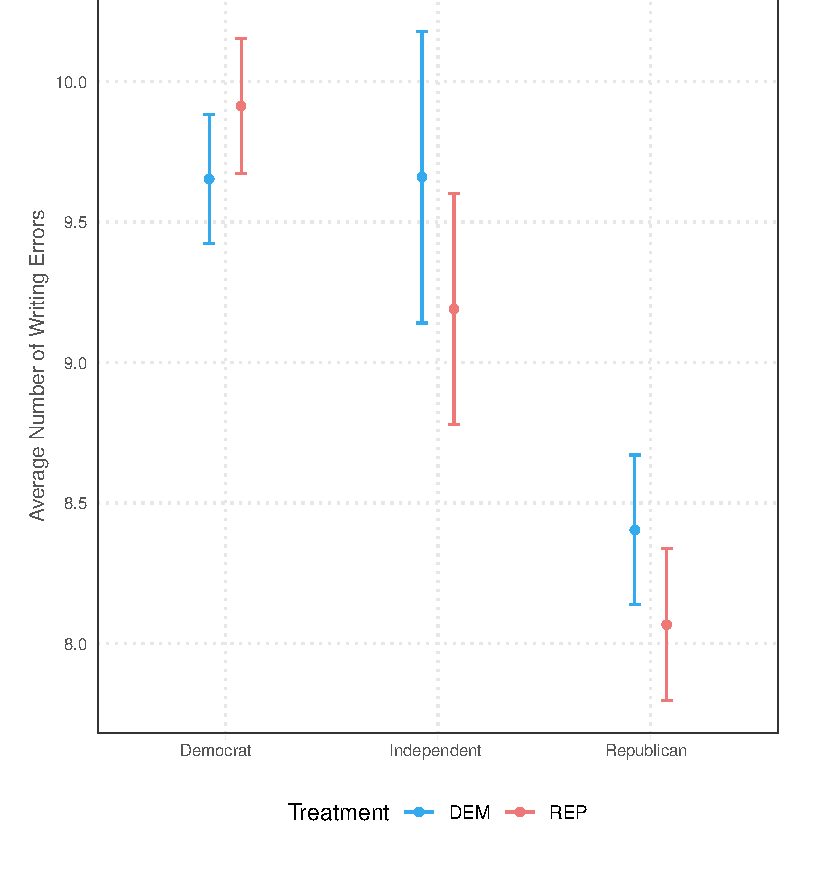
\includegraphics[]{../figs/text_cces.pdf}
\label{fig:text_cces}
\end{figure}
\clearpage
\begin{figure}[!htbp]
\centering
\caption{Writing Errors (Lucid)}
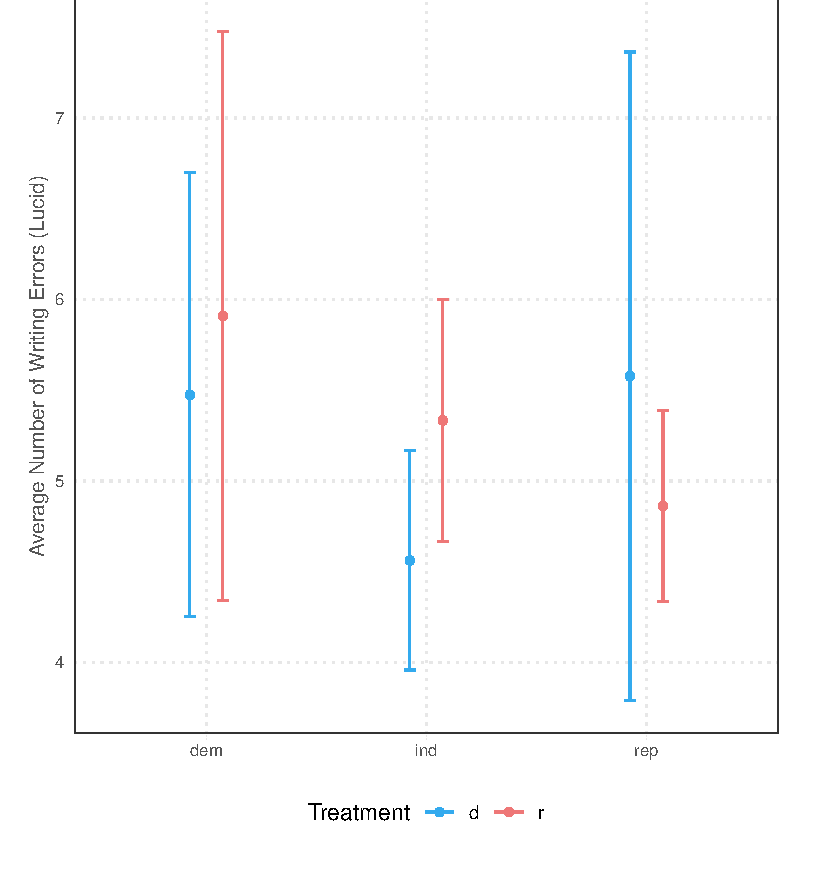
\includegraphics[]{../figs/text_lucid.pdf}
\label{fig:text_lucid}
\end{figure}

\clearpage
\begin{figure}[!htbp]
\centering
\caption{Poorly Parked Cars (CCES)}
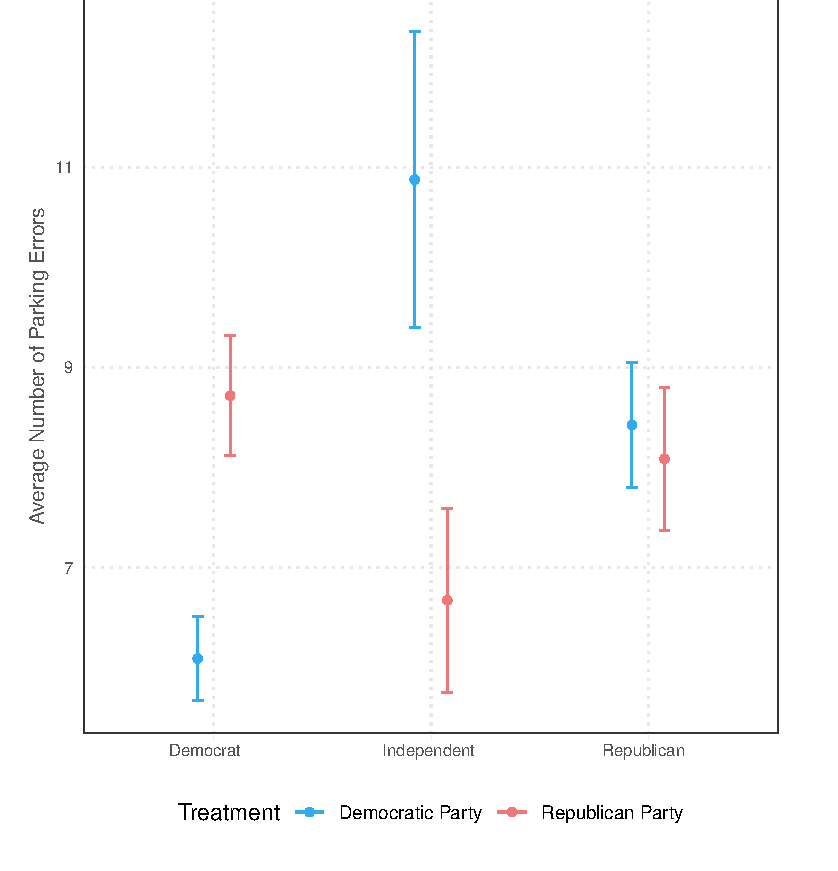
\includegraphics[]{../figs/parking_cces.pdf}
\label{fig:parking_cces}
\end{figure}


\end{document}